\documentclass[11pt,letterpaper]{article}
% --- Packages ---
\usepackage[utf8]{inputenc}
\usepackage[margin=1in]{geometry}
\usepackage{amsmath, amssymb, amsthm, amsfonts}
\usepackage{graphicx}
\usepackage{xcolor}
\usepackage{hyperref}
\usepackage{xurl}
\usepackage{booktabs}
\usepackage{cite}
\usepackage{microtype}
\usepackage{titlesec}
\usepackage{tcolorbox}
\usepackage{tikz}
\usetikzlibrary{arrows.meta, angles, quotes, snakes}
% --- Color Palette (De-saturated, Academic & Professional) ---
\definecolor{ajpblue}{RGB}{28, 54, 115}   % Deep navy accent
\definecolor{ajpsec}{RGB}{54, 95, 145}   % Secondary slate blue
\definecolor{bglight}{RGB}{245, 247, 250} % Light background for callout boxes
\definecolor{bordergrey}{RGB}{210, 215, 223}
% --- Hyperref Setup ---
\hypersetup{
colorlinks=true,
linkcolor=ajpblue,
citecolor=ajpsec,
urlcolor=ajpblue
}
% --- Typography & Headings Styling ---
\titleformat{\section}{\large\bfseries\color{ajpblue}}{\thesection}{1em}{}[{\titlerule[0.5pt]}]
\titleformat{\subsection}{\normalsize\bfseries\color{ajpsec}}{\thesubsection}{1em}{}
% --- Custom Environments for Explanation ---
\newtcolorbox{equationbreakdown}[1]{
colback=bglight,
colframe=ajpblue,
fonttitle=\bfseries,
title={Derivation Details \& Interpretation: #1},
arc=3pt,
boxrule=1pt,
bottomtitle=2mm,
toptitle=2mm
}
\newtcolorbox{physicsinsight}{
colback=bglight,
colframe=ajpsec,
boxrule=0.5pt,
left=4mm,
right=4mm,
top=3mm,
bottom=3mm,
arc=2pt
}
% --- Title & Project Metadata ---
\title{
\vspace{-1.5in}
\rule{\linewidth}{1.5pt} \\ \vspace{4mm}
\large\textbf{PHYSICS GROUP PROJECT REPORT} \\ \vspace{2mm}
\Large\textbf{An Explanatory Guide and Step-by-Step
Derivation of: \\ ``Oblique collision of a soft rubber disk with a rigid surface.''}
\\ \vspace{4mm}
\large\textit{Based on the Article in the American Journal of
Physics} \\
\rule{\linewidth}{1.5pt}
}
% Multi-column author format for a group project
\author{
\begin{tabular}{r @{\quad} l}
\textbf{Project Group:} & [rubber dynamics] \\[1ex]
\textbf{Group Members:} & Nayeon Kim (Report Preparation, Experimental Work \& Data Analysis) \\
& Yewon Kim: (Report Preparation, Presentation) \\
& Jisu Kang: (Presentation Design, Presentation) \\
& Yeju Kang: (Presentation Design, Experimental Work \& Data Analysis) \\[1ex]
\textbf{Course Title:}  & [General Physics] \\
\textbf{Instructor:}    & Dr. DEVECIOGLU DENIZ OLGU \\
\textbf{Department:}    & Department of Undergraduate Studies, \\
                        & DGIST (Daegu Gyeongbuk Institute of Science and Technology)
\end{tabular}
}
\date{June 16, 2026}
\begin{document}
\maketitle
\begin{abstract}
This project provides a comprehensive, pedagogical breakdown of the foundational paper ``Oblique collision of a soft rubber disk with a rigid surface'' by Rod Cross, published in the \textit{American Journal of Physics} (Volume 91, Pages 532--537, 2023) \cite{originalpaper}. While the original text assumes a certain level of mathematical and physical maturity, this report fills in the intermediate algebraic steps, explains the contextual physics principles, and interprets key equations. We reconstruct the derivations of the central models, analyze physical approximations, and discuss the implications of the results.
\end{abstract}
\tableofcontents
% =========================================================================
\section{Introduction \& Contextual Background}
% =========================================================================
\subsection{Historical and Pedagogical Significance}
This paper investigates the motion that occurs during the oblique collision of a soft rubber disk with a rigid surface.
While a collision is often simplified as an object hitting a surface and rebounding, the use of a soft rubber disk in this study means the object undergoes significant compression and deformation at the moment of impact.
Consequently, it is crucial to note that the disk does not merely bounce; instead, it rebounds while sliding and rotating.
This research serves as a practical application of core concepts from introductory physics---such as collision, friction, torque, and rotational motion---to a real-world scenario.
In particular, it illustrates how translational motion and rotational motion are interconnected, as the friction force acts to decrease the horizontal speed of the disk while simultaneously providing the torque that drives its rotation.
\subsection{Physical Setup and System Parameters}
When a soft rubber disk undergoes an oblique collision with a rigid surface, two primary forces act upon the disk. One is the normal reaction force ($N$), which the surface exerts upward on the disk, and the other is the friction force ($F$), which opposes the sliding of the disk along the surface.

\noindent The normal force causes the disk to rebound, while the friction force acts to decrease the horizontal speed of the object. Furthermore, because the friction force acts at the bottom contact patch of the disk, it provides the torque ($FR$) necessary to drive the disk's rotational motion.

\noindent In this context, $v_1$ and $v_2$ denote the speed of the center of mass before and after the collision, respectively. $v_{x1}$ and $v_{x2}$ are the horizontal velocity components of the center of mass. $R$ is the radius of the disk, $k_{||}$ is the stiffness parallel to the surface, $k_{\perp}$ is the stiffness in the vertical direction, and $\omega$ is the angular velocity about the center of mass.

\begin{figure}[h!]
\centering
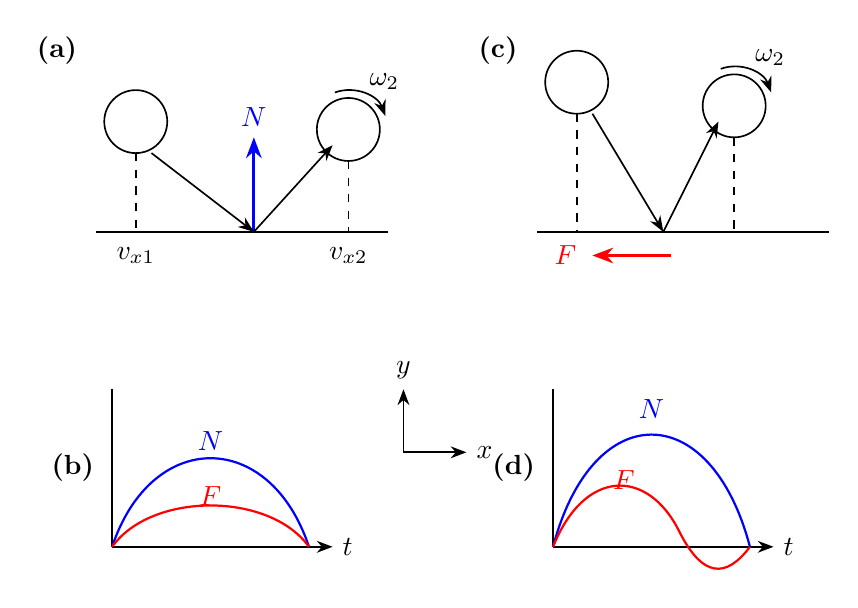
\begin{tikzpicture}[>=Stealth, line width=0.6pt]

    % Since I couldn't find the TeX file for the figure from the original paper, I recreated it to look identical and attached it as Figure 1.
    % ==========================================
    % (a) and (b) regions (left side)
    % ==========================================
    
    % (a) Drawing
    \node at (-0.7, 2.3) {\textbf{(a)}};
    
    % Ground line
    \draw (-0.2,0) -- (3.5,0);
    
    % Impact point and normal force N
    \coordinate (bounce1) at (1.8,0);
    \draw[blue, ->, line width=1pt] (bounce1) -- ++(0,1.2) node[above] {$N$};
    
    % Incoming ball and trajectory
    \draw (0.3,1.4) circle (0.4);
    \draw[dashed] (0.3,1.0) -- (0.3,0) node[below=2pt] {$v_{x1}$};
    \draw[->] (0.5,1.0) -- (bounce1);
    
    % Outgoing ball and trajectory
    \draw (3.0,1.3) circle (0.4);
    \draw[dashed] (3.0,0.9) -- (3.0,0) node[below=2pt] {$v_{x2}$};
    \draw[->] (bounce1) -- (2.8,1.1);
    
    % Rotation arrow omega_2
    \draw[->] (3.0,1.3) +(110:0.5) arc (110:20:0.5) node[midway, above right=-2pt] {$\omega_2$};

    
    % (b) Graph
    \begin{scope}[shift={(0,-1.5)}]
    \node at (-0.5, -1.5) {\textbf{(b)}};
    
    % Axes
    \draw[->] (0,-2.5) -- (2.8,-2.5) node[right] {$t$};
    \draw[-] (0,-2.5) -- (0,-0.5);
    
    % N curve (blue, high arch)
    \draw[blue, line width=0.8pt] (0,-2.5) .. controls (0.5,-1.0) and (2.0,-1.0) .. (2.5,-2.5);
    \node[blue, above] at (1.25,-1.4) {$N$};
    
    % F curve (red, low arch)
    \draw[red, line width=0.8pt] (0,-2.5) .. controls (0.5,-1.8) and (2.0,-1.8) .. (2.5,-2.5);
    \node[red, above] at (1.25,-2.1) {$F$};
    \end{scope}


    % ==========================================
    % Central coordinate axis symbols
    % ==========================================
    \begin{scope}[shift={(3.7,-2.8)}]
        \draw[->] (0,0) -- (0.8,0) node[right] {$x$};
        \draw[->] (0,0) -- (0,0.8) node[above] {$y$};
    \end{scope}


    % ==========================================
    % (c) and (d) regions (right side)
    % ==========================================
    \begin{scope}[shift={(5.6,0)}]
        
        % (c) Drawing
        \node at (-0.7, 2.3) {\textbf{(c)}};
        
        % Ground line
        \draw (-0.2,0) -- (3.5,0);
        
        % Impact point
        \coordinate (bounce2) at (1.4,0);
        
        % Incoming ball and trajectory (steeper)
        \draw (0.3,1.9) circle (0.4);
        \draw[dashed] (0.3,1.5) -- (0.3,0);
        \draw[->] (0.5,1.5) -- (bounce2);
        
        % Outgoing ball and trajectory
        \draw (2.3,1.6) circle (0.4);
        \draw[dashed] (2.3,1.2) -- (2.3,0);
        \draw[->] (bounce2) -- (2.1,1.4);
        
        % Rotation arrow omega_2
        \draw[->] (2.3,1.6) +(110:0.5) arc (110:20:0.5) node[midway, above right=-2pt] {$\omega_2$};
        
        % Friction force arrow F below ground
        \draw[red, <-, line width=1pt] (0.5,-0.3) node[left=2pt] {$F$} -- (1.5,-0.3);

        
        % (d) Graph
        \begin{scope}[shift={(0,-1.5)}]
        \node at (-0.5, -1.5) {\textbf{(d)}};
        
        % Axes
        \draw[->] (0,-2.5) -- (2.8,-2.5) node[right] {$t$};
        \draw[-] (0,-2.5) -- (0,-0.5);
        
        % N curve (blue, high arch)
        \draw[blue, line width=0.8pt] (0,-2.5) .. controls (0.5,-0.6) and (2.0,-0.6) .. (2.5,-2.5);
        \node[blue, above] at (1.25,-1.0) {$N$};
        
        % F curve (red, sinusoidal shape - transition from positive to negative)
        \draw[red, line width=0.8pt] (0,-2.5) 
            .. controls (0.4,-1.5) and (1.2,-1.5) .. (1.6,-2.3)
            .. controls (1.9,-2.9) and (2.2,-2.9) .. (2.5,-2.5);
        \node[red, above] at (0.9,-1.9) {$F$};
        \end{scope}
        
    \end{scope}

\end{tikzpicture}
\caption{Oblique angle collisions between a circular object and a horizontal surface showing the normal (N) and friction (F) forces vs time. (a) and (b) Glancing angle collisions. (c) and (d) A higher angle collision.}
\label{fig:sample_plot}
\end{figure}

\noindent Figure~\ref{fig:sample_plot} illustrates the behavior of the normal and friction forces during impact. The normal force acts upward, and the friction force acts in the horizontal direction. This figure clarifies that the interaction is not a simple bounce; rather, it involves a simultaneous change in horizontal velocity and the manifestation of rotational motion.

At a low angle of incidence, the lower vertical velocity results in minimal compression of the spring system before rebounding, which keeping the induced normal force $N$ relatively small. Conversely, a high angle of incidence introduces a substantially larger vertical velocity that drives the spring to its maximum deformation. In accordance with Hooke's law ($N = k_\perp y$), this pronounced compression consequently generates the peak normal force observed during the impact.

\begin{table}[h!]   
\centering
\caption{Physical Properties and Inertia}
\label{tab:physical_props}
\begin{tabular}{ll}
\toprule
\textbf{Symbol} & \textbf{Physical Meaning / Definition} \\
\midrule
$m$ & The mass of the rubber disk \\
$I_{cm}$ & The moment of inertia about the central axis ($I_{cm} = \alpha m R^2$) \\
$\alpha$ & The moment of inertia coefficient (1/2 for a uniform disk; 2/5 for a solid sphere) \\
$m_E$ & The effective mass of the bottom region ($m_E = m/(1+1/\alpha)$) \\
\bottomrule
\end{tabular}
\end{table}

\begin{table}[h!]
\centering
\caption{Motion State and Angles}
\label{tab:motion_state}
\begin{tabular}{ll}
\toprule
\textbf{Symbol} & \textbf{Physical Meaning / Description} \\
\midrule
$\theta_1, \theta_2$ & Incident and rebound angles relative to the horizontal surface \\
$v_{y1}, v_{y2}$ & Vertical velocity components of the CM before and after collision \\
$\omega_1, \omega_2$ & Angular velocity before and after the collision \\
$t, T$ & Time and total duration of the collision ($T = \pi/\omega_{\perp}$) \\
$t_0$ & Time when initial sliding phase ends and grip phase commences \\
$y$ & Vertical displacement of the center of mass \\
$x$ & Horizontal displacement (deformation) near the bottom of the disk \\
\bottomrule
\end{tabular}
\end{table}

\begin{table}[h!]
\centering
\caption{Modeling and Coefficients}
\label{tab:modeling_coeffs}
\begin{tabular}{ll}
\toprule
\textbf{Symbol} & \textbf{Physical Meaning / Formula} \\
\midrule
$\mu$ & Coefficient of sliding friction \\
$\omega_{\perp}$ & Angular frequency of vertical vibration ($\sqrt{k_{\perp}/m}$) \\
$\omega_k$ & Angular frequency of horizontal vibration ($\sqrt{k_{||}/m_E}$) \\
$N_0$ & Maximum value (amplitude) of the normal reaction force \\
$e_x$ & Tangential coefficient of restitution \\
COR & Normal coefficient of restitution ($-v_{y2}/v_{y1}$) \\
COF & Effective coefficient of friction (horizontal/vertical impulse ratio) \\
$S_2$ & Spin factor ($R\omega_2/v_{x2}$) \\
$\beta_1, \beta_2$ & Normalized angles of incidence and reflection for the contact point \\
\bottomrule
\end{tabular}
\end{table}

The key physical parameters are summarized in Tables~\ref{tab:physical_props}, \ref{tab:motion_state}, and \ref{tab:modeling_coeffs}.

% =========================================================================
\section{Step-by-Step Mathematical Derivations}
% =========================================================================
This section reconstructs the mathematical framework of the rubber disk collision, filling in the intermediate steps from the vertical motion to the final rebound state.

\begin{figure}[h!]
\centering
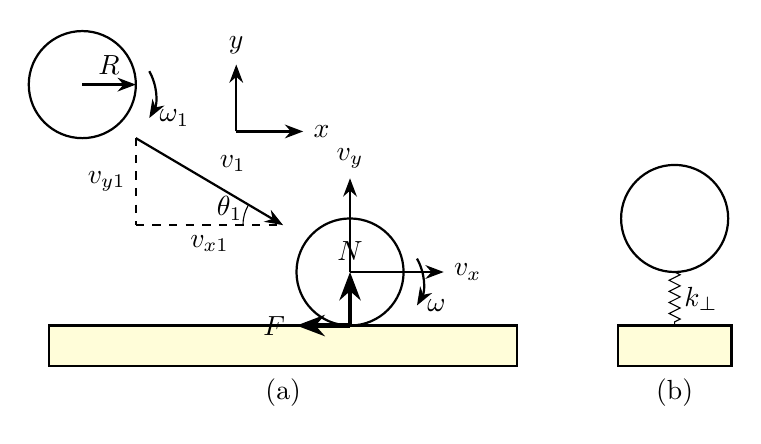
\begin{tikzpicture}[>=Stealth, scale=0.85]

    % Since I couldn't find the TeX file for the figure from the original paper, I recreated it to look identical and attached it as Figure 2.
    % ==========================================
    % Ground/Table
    % ==========================================
    \draw[fill=yellow!15, thick] (-4,-1) rectangle (3,-0.4);
    \node at (-0.5,-1.4) {(a)};
    
    \draw[fill=yellow!15, thick] (4.5,-1) rectangle (6.2,-0.4);
    \node at (5.35,-1.4) {(b)};

    % ==========================================
    % Coordinate System
    % ==========================================
    \begin{scope}[shift={(-1.2,2.5)}]
        \draw[->, thick] (0,0) -- (1,0) node[right] {$x$};
        \draw[->, thick] (0,0) -- (0,1) node[above] {$y$};
    \end{scope}

    % ==========================================
    % Figure (a) - Left ball (Falling)
    % ==========================================
    \coordinate (C1) at (-3.5, 3.2);
    \def\R{0.8}
    \draw[thick] (C1) circle (\R);
    \draw[->, thick] (C1) -- ++(\R,0) node[midway, above] {$R$};
    
    % 각속도 \omega_1 화살표
    \draw[->, thick] (-2.5, 3.4) arc (30:-30:0.7) node[right] {$\omega_1$};
    
    % 속도 벡터 및 삼각형
    \coordinate (V_start) at (-2.7, 2.4);
    \draw[->, thick] (V_start) -- ++(2.2, -1.3) node[midway, above right] {$v_1$};
    \draw[dashed, thick] (V_start) -- ++(0, -1.3) node[midway, left] {$v_{y1}$};
    \draw[dashed, thick] (-2.7, 1.1) -- ++(2.2, 0) node[midway, below] {$v_{x1}$};
    
    % 각도 \theta_1
    \draw (-1.1, 1.1) arc (180:150:0.6);
    \node at (-1.3, 1.35) {$\theta_1$};

    % ==========================================
    % Figure (a) - Right ball (Impact/On Surface)
    % ==========================================
    \coordinate (C2) at (0.5, 0.4);
    \draw[thick] (C2) circle (\R);
    
    % 속도 벡터들
    \draw[->, thick] (C2) -- ++(1.4, 0) node[right] {$v_x$};
    \draw[->, thick] (C2) -- ++(0, 1.4) node[above] {$v_y$};
    
    % 각속도 \omega
    \draw[->, thick] (1.5, 0.6) arc (30:-30:0.7) node[right] {$\omega$};
    
    % 힘 벡터 (N, F)
    \coordinate (Contact1) at (0.5, -0.4);
    \draw[->, ultra thick] (Contact1) -- ++(0, 0.8) node[above] {$N$};
    \draw[->, ultra thick] (Contact1) -- ++(-0.8, 0) node[left] {$F$};

    % ==========================================
    % Figure (b) - Ball with a spring
    % ==========================================
    \coordinate (C3) at (5.35, 1.2);
    \draw[thick] (C3) circle (\R);
    \draw[snake=zigzag, segment amplitude=2pt, segment length=4pt] (5.35, 0.4) -- (5.35, -0.4);
    \node[right] at (5.35, 0) {$k_{\perp}$};

\end{tikzpicture}
\caption{Schematic of variables and force components for (a) the oblique collision and (b) the stiffness model.}
\label{fig:collision_vars}
\end{figure}

\subsection{The Starting Framework: Vertical Simple Harmonic Motion (SHM)}
The first step in understanding the disk's motion is analyzing the vertical forces. The study models the vertical deformation of the disk during collision as a linear spring with stiffness $k_{\perp}$.

\noindent The vertical equation of motion is given by:
\begin{equation}
N = m \frac{d^2 y}{dt^2} = -k_{\perp} y
\end{equation}
This implies that the vertical motion of the disk behaves as Simple Harmonic Motion (SHM). Consequently, the normal force ($N$) as a function of time is:
\begin{equation}
N(t) = N_0 \sin(\omega_{\perp} t)
\end{equation}
where $\omega_{\perp} = \sqrt{k_{\perp}/m}$ is the angular frequency and $N_0$ is the maximum amplitude of the normal force.

\begin{physicsinsight}
\textbf{Physical Interpretation:} \\When the disk reaches maximum vertical compression, the vertical velocity $v_y$ becomes zero, and the normal force $N$ reaches its peak. Conversely, when there is no deformation, $N=0$.
\end{physicsinsight}

\subsection{Initial Sliding Phase: Velocity Changes Due to Friction}
At the beginning of the collision, the contact patch slides across the surface. In this sliding phase, the friction force $F$ is defined by:
\begin{equation}
F = \mu N(t)
\end{equation}
The friction force varies over time because $N(t)$ is time-dependent. The horizontal and rotational equations of motion are:
\begin{align}
F &= -m \frac{dv_x}{dt} \\
FR &= I_{cm} \frac{d\omega}{dt} \quad (\text{where } I_{cm} = \alpha m R^2)
\end{align}
Substituting $N(t)$ and integrating, we derive the horizontal velocity $v_x(t)$ during the collision:
\begin{equation}
v_x(t) = v_{x1} + \mu v_{y1} (1 - \cos \omega_{\perp} t)
\end{equation}

Vertical Modeling Condition: This equation is derived under the assumption that the vertical behavior at the moment of impact is not a rigid-body collision, but rather a linear spring system (harmonic oscillator) with a finite stiffness $k_\perp$.

\subsection{The Transition to Grip: Condition for Entering the Grip Phase}
As the collision progresses, the friction force causes $v_x$ to decrease and $R\omega$ to increase. The transition to the grip phase occurs when the relative velocity of the contact point vanishes:
\begin{equation}
v_x = R\omega
\end{equation}
Once this condition is met, an increase in the angle of incidence causes the disk to exert a greater downward force on the surface, thereby intensifying both the normal force and the friction force. Consequently, the bottom contact point of the disk momentarily becomes arrested, effectively coming to a near-instantaneous standstill as if pinned to the surface.

\subsection{Grip Phase and Reverse Sliding: Horizontal Deformation and Force Reversal}
The reverse sliding phase occurs toward the end of the collision when the stored horizontal elastic energy in the disk is released. During this stage, the kinematic relationship transitions to $v_x < R\omega$, meaning that while the center of mass continues to move forward ($v_x > 0$), the tangential speed of the contact point due to rotation ($R\omega$) is greater in the opposite direction. As a result, the contact patch slides backward (to the left) relative to the surface, causing the friction force ($F$) to reverse its original direction and act to the right. This reversed friction provides a final impulsive torque that further increases the disk's angular velocity. Consequently, the disk typically departs the surface in an overspinning mode, where the final tangential velocity of rotation exceeds the translational velocity of the center of mass ($R\omega_2 > v_{x2}$).

During the grip phase, sliding friction is replaced by a static restorative force:
\begin{equation}
F = k_{||} x
\end{equation}
To describe the horizontal deformation, the model introduces an effective mass $m_E$:
\begin{equation}
m_E = \frac{m}{1 + 1/\alpha}
\end{equation}
\noindent Toward the end of the collision, the stored elastic energy causes the friction force to reverse direction (reverse sliding). This restorative force results in the disk rebounding with a significantly increased spin.

\subsection{Concluding Parameter: Tangential Coefficient of Restitution ($e_x$)}
The final post-collision state is determined by the tangential coefficient of restitution, $e_x$, defined as:
\begin{equation}
e_x = \frac{R\omega_2 - v_{x2}}{v_{x1}}
\end{equation}
When the incident angle is approximately $23^\circ$ or higher, the grip phase becomes prominent, and $e_x$ typically reaches a value of about 0.5. This mathematically demonstrates that the horizontal deformation of the rubber disk plays a vital role in the collision outcome.

% =========================================================================
\section{Physical Approximations and Limiting Cases}
% =========================================================================

\subsection{Simplified Models and Physical Approximations}
While the actual collision of a soft rubber disk is highly complex, the paper presents a simplified model to facilitate a pedagogical understanding. The primary simplification involves dividing the collision process into three separate stages: the initial sliding phase, the subsequent grip phase, and the final (reverse) sliding phase.

\noindent Furthermore, because the rubber disk undergoes significant deformation during impact, the study models the disk's behavior using linear springs. In the normal (vertical) direction, the disk is compressed, generating a normal reaction force ($N$). In the tangential (horizontal) direction, while the contact patch is held at rest, the disk undergoes horizontal shear or stretching.

\noindent Specifically, during the grip phase, although the contact patch remains stationary on the surface, the upper portion of the disk continues its forward motion due to inertia. This results in a horizontal deformation of the disk, a characteristic that distinguishes it from the collision of a perfectly rigid body.

\noindent The collision dynamics also vary according to the angle of incidence. At glancing angles of incidence, the disk strikes the surface at a shallow angle. In this case, the normal and friction forces are insufficient to stop the sliding, so the disk primarily continues to slide throughout the collision. Conversely, at higher angles of incidence, the disk exerts a stronger force on the surface, leading to increased normal and friction forces. This causes the contact point to momentarily stop, entering the grip phase, which subsequently results in a significant increase in the disk's outgoing spin.

% =========================================================================
\section{Experimental Methods and Analysis}

\subsection{Experiment Background}

\subsubsection*{Material and Apparatus Limitations}
Since the identical Chutex rubber disk utilized in the reference literature was unavailable for purchase, an alternative product was selected for this study. The alternative rubber disk consists of a more rigid material with higher hardness compared to the original Chutex disk. Consequently, as noted in the reference study, it was challenging to observe significant horizontal deformation under high angles of incidence. The motion of the disk during impact was captured using a high-speed camera operating at 240 frames per second (fps), and the recorded footage was quantitatively analyzed using the Tracker video analysis software.

\subsubsection*{Experimental Setup}
The experimental procedure was established through the following protocols:
\begin{itemize}
    \item A 15 cm ruler was vertically installed within the camera's field of view to define the reference scale factor.
    \item The center of mass (CoM) was marked on a rubber disk with a thickness of 20 mm and a radius of 36 mm using a white marker.
    \item Four distinct points were marked along the circumference of the disk at $90^{\circ}$ intervals to track and verify the rotational motion relative to the center.
    \item To prevent any unwanted camera movement or vibration induced by the impact, the camera was mounted on a separate structure decoupled from the impact platform.
    \item A target impact zone optimized for camera recording was designated on the impact platform, and the rubber disk was manually launched toward this target area.
\end{itemize}
Due to the absence of a precision mechanical launcher capable of fine angular adjustments, the disk was thrown manually, which resulted in non-uniform intervals between the collected incident angles. Consequently, out of the total recorded videos, datasets captured at specific angles ($34.2^{\circ}$, $37.6^{\circ}$, $39.5^{\circ}$, and $48.0^{\circ}$) were selected for evaluation. In this study, while data were collected across all four angles, a detailed kinematic and dynamic analysis was conducted on three representative angles: $34.2^{\circ}$, $39.5^{\circ}$, and $48.0^{\circ}$.

\subsubsection*{Video Tracking and Data Extraction Process}
The kinematic parameters were extracted through the Tracker analysis software using the following sequential steps:
\begin{itemize}
    \item The center of mass was designated as Point Mass A, and its trajectory was tracked frame by frame.
    \item With the origin of the coordinate system set at the bottom-left corner of the video frame, the pre- and post-collision velocities of the center of mass (Point Mass A) along the $x$- and $y$-axes were recorded.
    \item The pre-collision velocity was defined by averaging the velocities collected prior to the impact, and the post-collision velocity was similarly defined by averaging the velocities recorded after the impact.
    \item One of the four points marked on the circumference was designated as Point Mass B, and its motion was tracked frame by frame.
    \item Setting the center of mass (Point Mass A) as a moving origin, the post-collision angular velocity of Point Mass B relative to the center of mass was recorded.
    \item The post-collision angular velocity was defined by averaging the angular velocities collected during the post-impact phase.
    \item The angle of incidence was determined by measuring the angle between the pre-impact trajectory of the center of mass and the horizontal datum plane using the protractor function within the Tracker software.
\end{itemize}

(The raw data, original experimental videos, and Tracker analysis files are available on the GitHub repository \cite{githubrepo}.)

\begin{figure}[h!]
\centering

\includegraphics[width=0.8\linewidth]{images/image.png}
\caption{Visual representation of the video tracking and data extraction process using Tracker software.}
\label{fig:tracker_interface}
\end{figure}

\begin{table}[h!]
\centering
\caption{Raw kinematic data for the four experimental videos extracted via Tracker software.}
\label{tab:tracker_raw_data}
\resizebox{\textwidth}{!}{
\begin{tabular}{lccccccc}
\toprule
\textbf{Source} & \textbf{Angle ($^\circ$)} & \textbf{$v_{x1}$ (m/s)} & \textbf{$v_{x2}$ (m/s)} & \textbf{$v_{y1}$ (m/s)} & \textbf{$v_{y2}$ (m/s)} & \textbf{$\omega_2$ (rad/s)} & \textbf{$R$ (m)} \\
\midrule
Video 1 & 37.6 & 7.63475975 & 4.450893875 & -6.98414975 & 3.559969333 & -76.26846580 & 0.036 \\
Video 2 & 48.0 & 127.76346670 & 86.93571667 & -88.43719000 & 53.59178667 & -82.71145287 & 0.036 \\
Video 3 & 39.5 & 8.66088275 & 6.667978600 & -7.87184400 & 3.980195200 & -72.30429161 & 0.036 \\
Video 4 & 34.2 & 7.21453750 & 4.379404333 & -4.61954525 & 2.966339333 & -87.94129665 & 0.036 \\
\bottomrule
\end{tabular}
}
\end{table}

\subsection{Collision at an Incident Angle of 34.2$^\circ$}
$$ \text{COR} = -\frac{v_{y2}}{v_{y1}} = -\frac{2.966339}{-4.61955} \approx 0.6421 $$
The coefficient of restitution ($\text{COR}$) was calculated as $0.6421$, indicating that the post-collision vertical speed is approximately 64.21\% of the pre-collision vertical speed. This result is slightly lower than the value of 0.72 presented in the literature for high angles of incidence.

$$ \text{COF} = \frac{7.214538 - 4.379404}{2.966339 - (-4.61955)} = 0.37373787031 \approx 0.374 $$
The effective coefficient of friction ($\text{COF}$) indicates that the tangential impulse is approximately $37.4\%$ of the normal impulse, reflecting the frictional resistance during the impact at this specific angle.

\noindent The linear velocity at the contact point induced by rotation is:
$$ R|\omega_2| = (0.036)(87.9413) = 3.1658868 \text{ m/s} $$

\vspace{1em}
$$ S_2 = \frac{R|\omega_2|}{v_{x2}} = \frac{3.1658868}{4.379404} = 0.72290357318 \approx 0.723 $$

\vspace{1em}
\noindent Since $S_2 < 1$, the rightward translational velocity of the center of mass is greater than the leftward linear velocity at the contact point induced by rotation.

$$ e_x = \frac{3.1658868 - 4.379404}{7.214538} = -0.16820439507 \approx -0.168 $$
\subsection{Collision at an Incident Angle of 39.5$^\circ$}
$$ \text{COR} = -\frac{v_{y2}}{v_{y1}} = -\frac{3.560}{-6.984} = 0.512342599 \approx 0.512 $$
The normal coefficient of restitution ($\text{COR}$) was calculated as $0.512$, indicating that the post-impact normal speed is approximately $51\%$ of its pre-impact value. This confirms that the collision is inelastic, where a significant portion of the normal kinetic energy was dissipated through deformation, heat, and acoustic radiation.

Compared with the reference literature, which reported a $\text{COR}$ of approximately $0.72$ at angles of incidence greater than $20^\circ$, the experimental value obtained in this study ($0.51$) is notably lower. This discrepancy can be attributed to differences in the material properties of the surface and the disk, as well as variations in deformation behavior and energy dissipation mechanisms.

$$ \text{COF} = \frac{7.63476 - 4.450894}{3.559969 - (-6.98415)} = 0.30195656934 \approx 0.302 $$
The post-impact tangential impulse was approximately $30.2\%$ of the normal impulse. Furthermore, the tangential velocity decreased from $7.63476\text{ m/s}$ to $4.450894\text{ m/s}$, confirming that the frictional force acted to reduce the horizontal translational motion of the disk.

\noindent The linear velocity at the contact point induced by rotation is calculated as follows:
$$ R|\omega_2| = (0.036)(76.2685) = 2.745666 \text{ m/s} $$

\vspace{1em}
$$ S_2 = \frac{R|\omega_2|}{v_{x2}} = \frac{2.745666}{4.450894} \approx 0.617 $$

\vspace{1em}
\noindent Therefore, the slip velocity at the contact point immediately after the collision is calculated as $4.450894 - 2.745666 = 1.705228\text{ m/s}$.

$$ e_x = \frac{2.745666 - 4.450894}{7.63476} = \frac{-1.705228}{7.63476} = -0.22335057029 \approx -0.223 $$

\subsection{Collision at an Incident Angle of 48$^\circ$}
% COR calculation and explanation for 4.3
$$ \text{COR} = -\frac{v_{y2}}{v_{y1}} = -\frac{53.59179}{-88.4372} = 0.60598696024 \approx 0.606 $$
Since the post-collision vertical speed is approximately 60.6\% of the pre-collision vertical speed, the remaining energy is dissipated in the form of material deformation, heat, and acoustic emissions. This result confirms the inelastic nature of the collision at this higher angle of incidence.

$$ \text{COF} = \frac{127.7635 - 86.93572}{53.59179 - (-88.4372)} = 0.28746089091 \approx 0.287 $$
The effective coefficient of friction ($\text{COF}$) indicates that the tangential impulse is approximately $28.7\%$ of the normal impulse, reflecting the frictional resistance during the impact at this specific angle.

\noindent The linear velocity at the contact point induced by rotation is:
$$ R|\omega_2| = (0.036)(82.7115) = 2.977614 \text{ m/s} $$

$$ S_2 = \frac{R|\omega_2|}{v_{x2}} = \frac{2.977614}{86.93572} = 0.03425075447 \approx 0.0343 $$
Given that the linear velocity at the contact point induced by rotation is approximately $2.98\text{ m/s}$ and the horizontal velocity of the center of mass is roughly $86.94\text{ m/s}$, the translational motion is highly dominant.

$$ e_x = \frac{2.977614 - 86.93572}{127.7635} = -0.65716034705 \approx -0.657 $$

\subsection{Experiment result}
The coefficients of restitution ranged from 0.51 to 0.64 and did not show a clear monotonic dependence on the incident angle. The effective coefficient of friction decreased as the incident angle increased. At $34.2^\circ$ and $37.6^\circ$, $S_2 < 1$, indicating that translational motion remained dominant and reverse sliding was not clearly observed. However, the $48^\circ$ data likely contain a unit inconsistency. After correcting the velocity units, $S_2$ becomes greater than 1, supporting the transition to overspin and reverse sliding at a higher incident angle.
% =========================================================================
\section{Critical Analysis and Commentary}
% =========================================================================
The primary strength of this research lies in its approach to collision not merely as an instantaneous change in velocity, but as a complex process where translational motion, rotational motion, friction, and the deformation of the rubber disk interact simultaneously. While standard introductory physics problems often focus only on pre- and post-impact velocity vectors, this study emphasizes that surface friction and material deformation are critical to understanding real-world impacts.

\noindent Specifically, the study effectively demonstrates how the friction force ($F$) serves as the link between translational and rotational motion. During the oblique collision, the friction force acts to decrease the horizontal velocity ($v_x$) of the center of mass while simultaneously generating a torque ($FR$) at the contact patch, which increases the disk's angular velocity ($\omega$). This illustrates the physical process by which a portion of the disk’s linear kinetic energy is converted into rotational energy.

\noindent Furthermore, the paper highlights that the horizontal (tangential) deformation of the rubber disk significantly influences the final outcome of the bounce. While it is common to consider only vertical (normal) deformation in bouncing scenarios, this research explains that during the grip phase, the disk undergoes significant horizontal shear. This elastic deformation leads to a reversal of the friction force (reverse sliding) toward the end of the impact, which substantially affects the magnitude of the outgoing spin.

\noindent Ultimately, this study proves that modeling real-world collisions simply as rigid body interactions is insufficient. To achieve a comprehensive understanding of the dynamics, it is essential to account for the intricate interplay between friction and elastic deformation.

% =========================================================================
\section{Conclusion}
% =========================================================================
This project has provided a comprehensive pedagogical breakdown of the complex dynamics involved in the oblique collision of a soft rubber disk. The key insights gained from this analysis are summarized below:
\begin{itemize}
    \item An oblique collision is a continuous interaction of \textbf{translation, rotation, friction, and elastic deformation}, rather than a simple instantaneous bounce.
    \item Friction decreases the horizontal velocity while generating torque, thereby converting part of the translational motion into rotational motion.
    \item At sufficiently high incident angles, the collision proceeds through three stages: \textbf{initial sliding $\rightarrow$ grip $\rightarrow$ reverse sliding}.
    \item Horizontal deformation during the grip phase stores elastic energy and can reverse the direction of friction, producing increased spin after the collision.
    \item By reconstructing the intermediate derivations, this project clarified how the mathematical model represents the physical behavior of a deformable rubber disk.
\end{itemize}
% =========================================================================
\begin{thebibliography}{99}
\sloppy
% =========================================================================
\bibitem{originalpaper}
Cross, R. (2023). ``Oblique collision of a soft rubber disk with a rigid surface.'' \textit{American Journal of Physics}, 91(7), 532--537.

\bibitem{githubrepo}
Kim, N. (2026). ``Derivation and explanation: Oblique collision of a soft rubber disk with a rigid surface.'' GitHub Repository. \url{https://github.com/Na-yeon-Kim/Derivation-and-explanation-Oblique-collision-of-a-soft-rubber-disk-with-a-rigid-surface}.
\end{thebibliography}
\end{document}
